\documentclass[]{article}
\usepackage[utf8]{inputenc}
\usepackage{hyperref}
\usepackage[spanish]{babel}
\usepackage{listings}
\usepackage{xcolor} %para el texto con coloresç
\usepackage{tocloft}
\usepackage{graphicx}

\usepackage[colorinlistoftodos,prependcaption,textsize=tiny]{todonotes}

\renewcommand{\cftsecleader}{\cftdotfill{\cftdotsep}} % Para que todo el índice tenga puntos
\newcommand{\code}[1]{{\lstinline[basicstyle=\ttfamily,mathescape]!#1!}}
\newcommand{\toolname}{\emph{Tutoriales Interactivos}}

\lstset{ %
	%backgroundcolor=\color{white},  % choose the background color; you must add \usepackage{color} or \usepackage{xcolor}
	basicstyle=\sffamily,      % the size of the fonts that are used for the code
	breakatwhitespace=false,         % sets if automatic breaks should only happen at whitespace
	breaklines=true,                 % sets automatic line breaking
	captionpos=none,                 % sets the caption-position to bottom
	commentstyle=\itshape\color{gray},           % comment style
	%deletekeywords={...},           % if you want to delete keywords from the given language
	escapeinside={(*}{*)},           % if you want to add LaTeX within your code
	extendedchars=true,              % lets you use non-ASCII characters; for 8-bits encodings only, does not work with UTF-8
	frame=tb,	                   % adds a frame around the code
	keepspaces=true,                 % keeps spaces in text, useful for keeping indentation of code (possibly needs columns=flexible)
	columns=fullflexible,
	%keywordstyle=\color{blue},      % keyword style
	keywordstyle=\sffamily\color{teal},
	numbers=left,                    % where to put the line-numbers; possible values are (none, left, right)
	numbersep=5pt,                   % how far the line-numbers are from the code
	numberstyle=\tiny, % the style that is used for the line-numbers
	%rulecolor=\color{black},         % if not set, the frame-color may be changed on line-breaks within not-black text (e.g. comments (green here))
	showspaces=false,                % show spaces everywhere adding particular underscores; it overrides 'showstringspaces'
	showstringspaces=false,          % underline spaces within strings only
	showtabs=false,                  % show tabs within strings adding particular underscores
	stepnumber=1,                    % the step between two line-numbers. If it's 1, each line will be numbered
	stringstyle=\color{blue},     % string literal style
	tabsize=2,	                   % sets default tabsize to 2 spaces
	title=\lstname,                   % show the filename of files included with \lstinputlisting; also try caption instead of title	
	mathescape=true
}

% Title Page
\title{\toolname{} - Manual de usuario \\ \emph{(Borrador)}}
\author{Enrique Martín Martín$^a$ (\url{emartinm@ucm.es}) \\ 
	Salvador Tamarit$^b$ (\url{stamarit@dsic.upv.es}) \\
	\emph{Revisor:} Jaime Sánchez Hernández$^a$ (\url{jaime@sip.ucm.es}) \\~\\[-.4cm]
	\normalsize{\emph{$^a$Dpto. de Sistemas Informáticos y Computación}}\\[-0.1cm]
	\normalsize{\emph{Fac. Informática, Universidad Complutense de Madrid}}\\[-0.1cm]
	%\normalsize{\emph{C/ Profesor José García Santesmases, 9. 28040 Madrid, Spain}}\\[-0.1cm]
	\normalsize{\emph{$^b$Dep. Sistemes Informàtics i Computació}}\\[-0.1cm]
	\normalsize{\emph{Universitat Politècnica de València}}\\[-0.1cm]
	%\normalsize{\emph{Camí de Vera, s/n. 46022 València}}\\[-0.1cm]
}


\begin{document}
\maketitle

\tableofcontents

\clearpage

\section{Instalación y ejecución}\todo{Enrique}

Para poder ejecutar la herramienta \toolname{} debéis tener instalada en vuestro sistema la última versión de Java (en el momento de escribir este manual es la \emph{versión 8 update 131)}. Para ello debéis acceder a la página \url{https://www.java.com/es/download/} y seguir las instrucciones.

Una vez disponemos de la última versión de Java, la instalación de la herramienta \toolname{} es muy sencilla: únicamente es necesario descargar el programa junto con las lecciones y situarlo en alguna carpeta del sistema (por ejemplo el directorio personal o el escritorio). Si vais a utilizar \toolname{} es una asignatura, lo más probable es que el profesor os proporcione un fichero comprimido con todos los elementos incorporados. En el caso de no disponer de este fichero comprimido proporcionado por el profesor, podéis descargar la herramienta de su repositorio oficial: \url{https://github.com/emartinm/TutorialesInteractivos/archive/master.zip}.
% y descomprimirlo en alguna carpeta del sistema\footnote{Si disponéis del sistema de control de versiones \emph{GIT} también podréis clonar el repositorio de la herramienta  usando la dirección \url{https://github.com/emartinm/TutorialesInteractivos.git}}.

Para ejecutar la herramienta, únicamente hay que hacer doble clic en el fichero \texttt{TutorialesInteractivos-jar-with-dependencies.jar} situado en la carpeta \texttt{target} dentro del directorio principal de la herramienta. En caso de no poder iniciar la herramienta de esta manera consulta la sección~\ref{sec:problemas_arrancar}.

\section{Configuración de la aplicación}\todo{Enrique}
\label{sec:configuracion}

La primera vez que se inicia la herramienta se acceder directamente a la ventana de configuración (ver figura~\ref{fig:config1}).
%
\begin{figure}[tbp]
	\begin{center}
		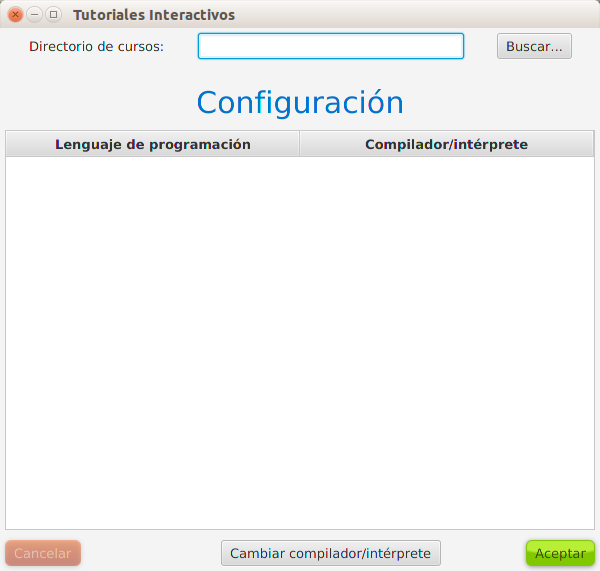
\includegraphics[scale=0.4]{Configuracion_vacia.png}
	\end{center}
	\caption{Ventana inicial de configuración\label{fig:config1}}
\end{figure}
%
En esta ventana lo primero que hay que hacer es configurar el \textbf{directorio de temas} pulsando el botón \emph{Buscar\ldots} que aparece aparece en la parte superior derecha. El directorio de temas normalmente se encuentra dentro del directorio principal de la herramienta, contiene carpetas por cada uno de los lenguajes disponibles: Python 3.x, C++, Java, etc. 

Tras configurar el directorio de temas, nos aparecerán varias entradas en el listado central de la ventana de configuración para establecer los compiladores o intérpretes para cada lenguaje disponible (ver figura~\ref{fig:config2}).
%
\begin{figure}[tbp]
	\begin{center}
		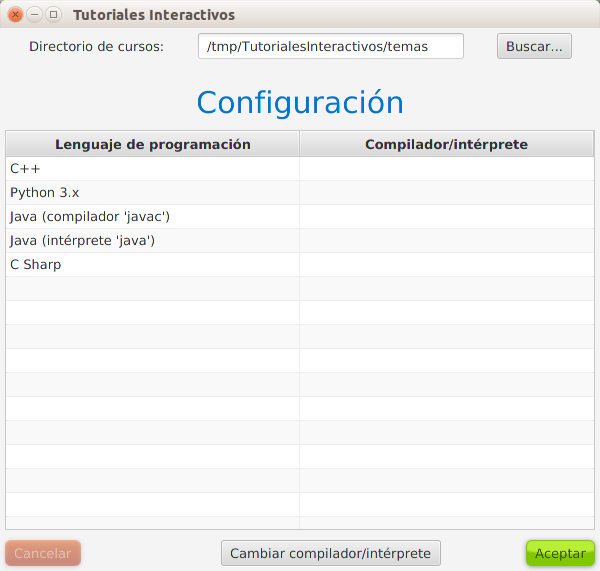
\includegraphics[scale=0.4]{Configuracion_lenguajes_vacio.png}
	\end{center}
	\caption{Ventana inicial de configuración con directorio de temas\label{fig:config2}}
\end{figure}
%
\begin{itemize}
	\item \textbf{Python 3.x}: debes establecer la ruta del \textbf{intérprete} de Python versión 3.x. En entornos Linux suele estar en \texttt{/usr/bin/python3}, aunque también se puede utilizar el binario instalado por \emph{Anaconda}. En entornos Windows el binario suele llamarse \texttt{python.exe} o \texttt{python3.exe}.
	\item \textbf{C++}: debes establecer la ruta del compilador de C++. En entornos Linux se utilizará el compilador GNU C++ que suele estar en la ruta \texttt{/usr/bin/g++}. En entornos Windows se puede utilizar GNU C++, pero también se soporta el compilador de C++ incluido en \emph{Visual Studio}. En este caso debes establecer la ruta del \emph{script} \texttt{vcvars32.bat} o \texttt{vcvars64.bat} (dependiendo de si el sistema es de 32 o 64 bits) que establecen las variables de entorno necesarias para compilar con \emph{Visual Studio}. La herramienta \toolname{} usará estas variables de entorno para encontrar el compilador de C++ (\texttt{cl.exe}) adecuado. La ruta de estos \emph{scripts} puede variar entre distintas versiones de \emph{Visual Studio} o entre versiones de Windows, por lo que recomendamos usar el buscador de ficheros para encontrarlos. Como ejemplos, en un sistema \emph{Windows 10} y para la versión \emph{Visual Studio 2013} estos ficheros están en la carpeta: \\[0.2cm]
	\texttt{C:\textbackslash Program Files (x86)\textbackslash Microsoft Visual Studio 12.0\textbackslash VC\textbackslash bin}\\[0.2cm]
	mientras que para la versión \emph{Visual Studio 2017} están en:\\[0.2cm]
	\texttt{C:\textbackslash Program Files (x86)\textbackslash Microsoft Visual Studio\textbackslash 2017\textbackslash \\% Professional \textbackslash\\ 
		Professional\textbackslash VC\textbackslash Auxiliary\textbackslash Build}.
	\item \textbf{C\#}: debes establecer la ruta del compilador de C\#. En el caso de usar \emph{Mono} es la ruta del fichero \texttt{mcs} o \texttt{mcs.exe}, que en sistemas Linux suele estar en \texttt{/usr/bin/mcs}. En sistemas Windows también se puede utilizar el compilador \texttt{csc.exe} de Visual Studio. En este último caso la ruta que hay que configurar es la del \emph{script} \texttt{vcvars32.bat} o \texttt{vcvars64.bat}, al igual que en el caso de C++.
	\item \textbf{Java}: ........
\end{itemize}
Al finalizar la configuración de la herramienta, la ventana debe tener un aspecto similar al mostrado en la figura~\ref{fig:config3}.
%
\begin{figure}[tbp]
	\begin{center}
		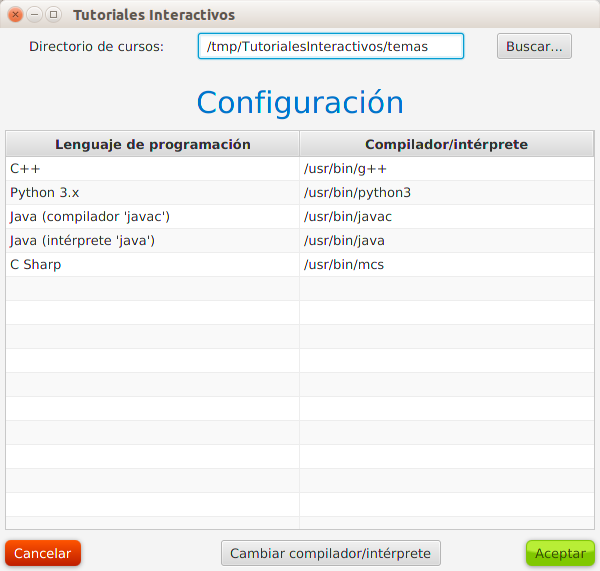
\includegraphics[scale=0.4]{Configuracion_lenguajes_relleno.png}
	\end{center}
	\caption{Ventana final de configuración, con las rutas usuales en entornos Linux\label{fig:config3}}
\end{figure}
%
Ten en cuenta que \textbf{no es obligatorio configurar los compiladores o intérpretes de todos los lenguajes de programación disponibles}, únicamente de aquellos que vayas a utilizar para realizar tutoriales.

\section{Navegación general}\todo{Tama}
\label{sec:ng}
Tras configurar la herramienta, como se describe en la sección \ref{sec:configuracion}, ya estará lista para ser utilizada. La siguiente ventana que se cargará será la de selección de lenguaje, como se muestra en la figura \ref{fig:ng_1}. En esta ventana se mostrarán todos los lenguajes disponibles, en este caso cuatro. Primero, deberemos seleccionar el lenguaje que queramos aprender. Tras la selección deberemos pulsar el botón \emph{Comenzar} para acceder a los temas disponibles para el lenguaje seleccionado. Desde la ventana de selección de lenguajes también se puede volver a los ajustes, descritos en la sección \ref{sec:configuracion}, mediante el botón \emph{Ajustes}.

%
\begin{figure}[tbp]
\begin{center}
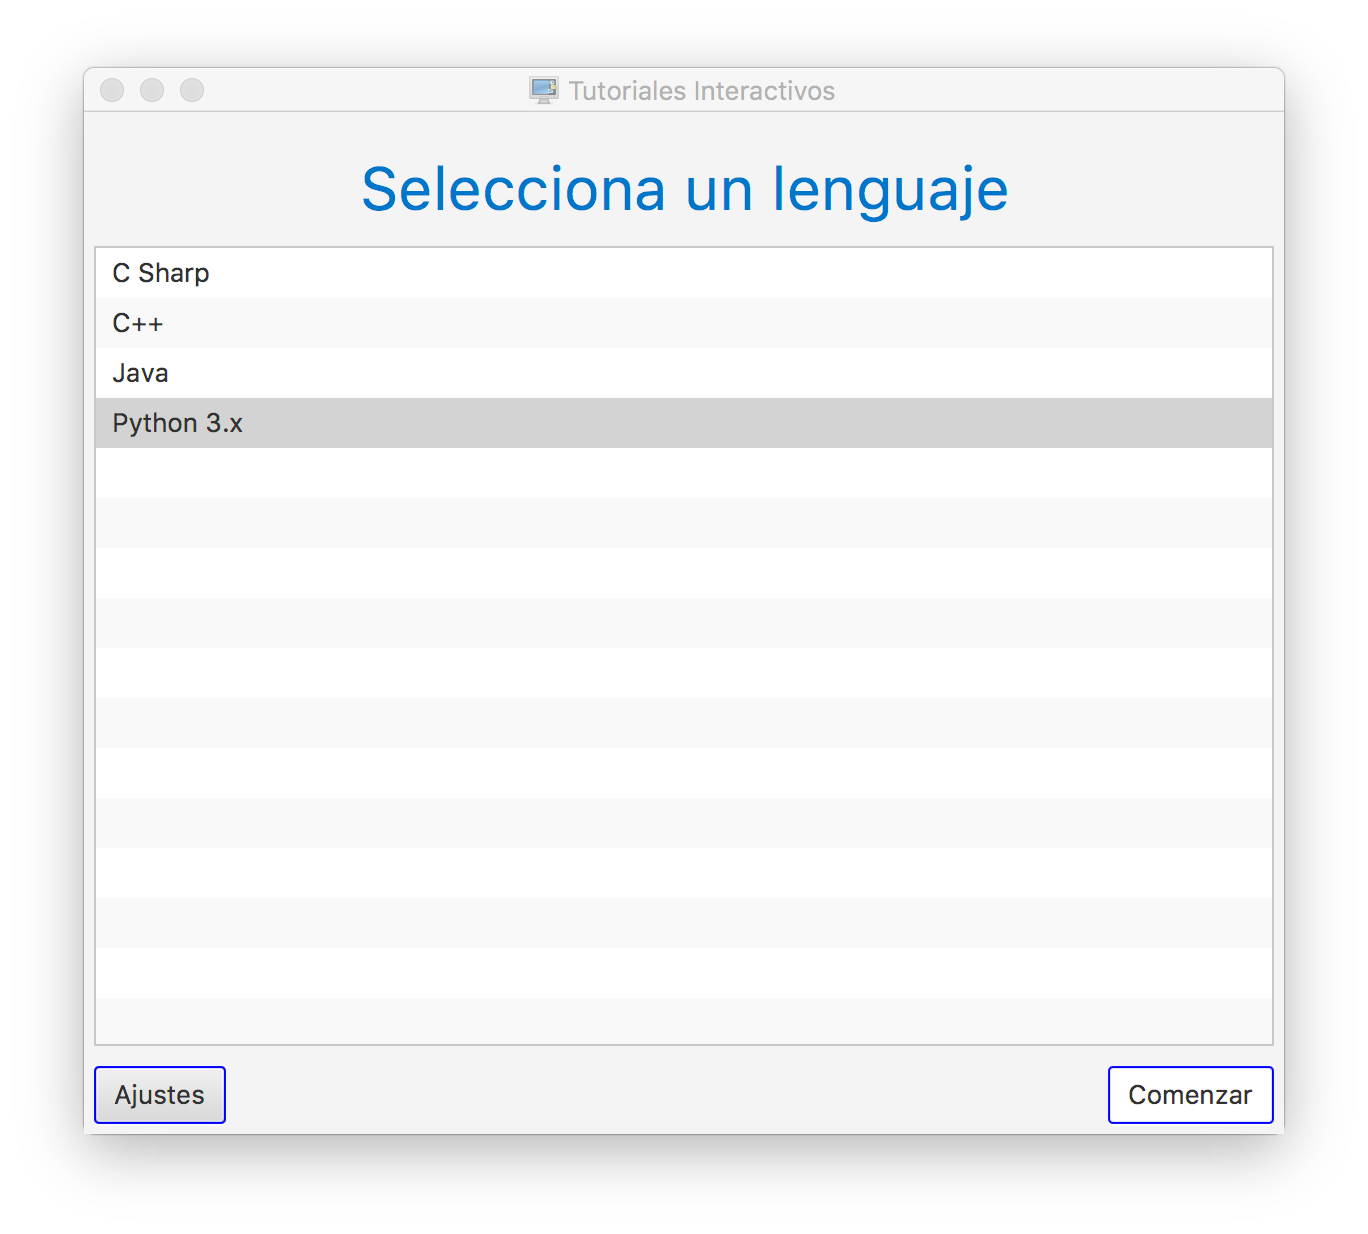
\includegraphics[scale=0.35]{ng_1.png}
\end{center}
\caption{Ventana de selección de lenguaje\label{fig:ng_1}}
\end{figure}
%

La ventana con los temas es como la que se muestra en la figura \ref{fig:ng_2}. Aquí deberemos de seleccionar alguno de los temas disponibles, en este caso solo hay uno, y darle al botón \emph{Comenzar}. Podremos también volver a la ventana de selección de lenguajes mediante el botón \emph{Volver}. Al lado de cada tema podemos observar el tanto por ciento del tema que se ha completado hasta el momento. Un ejemplo de como se mostraría un tema que se avanzado parcialmente se puede ver en la figura \ref{fig:ng_3}.

%
\begin{figure}[tbp]
\begin{center}
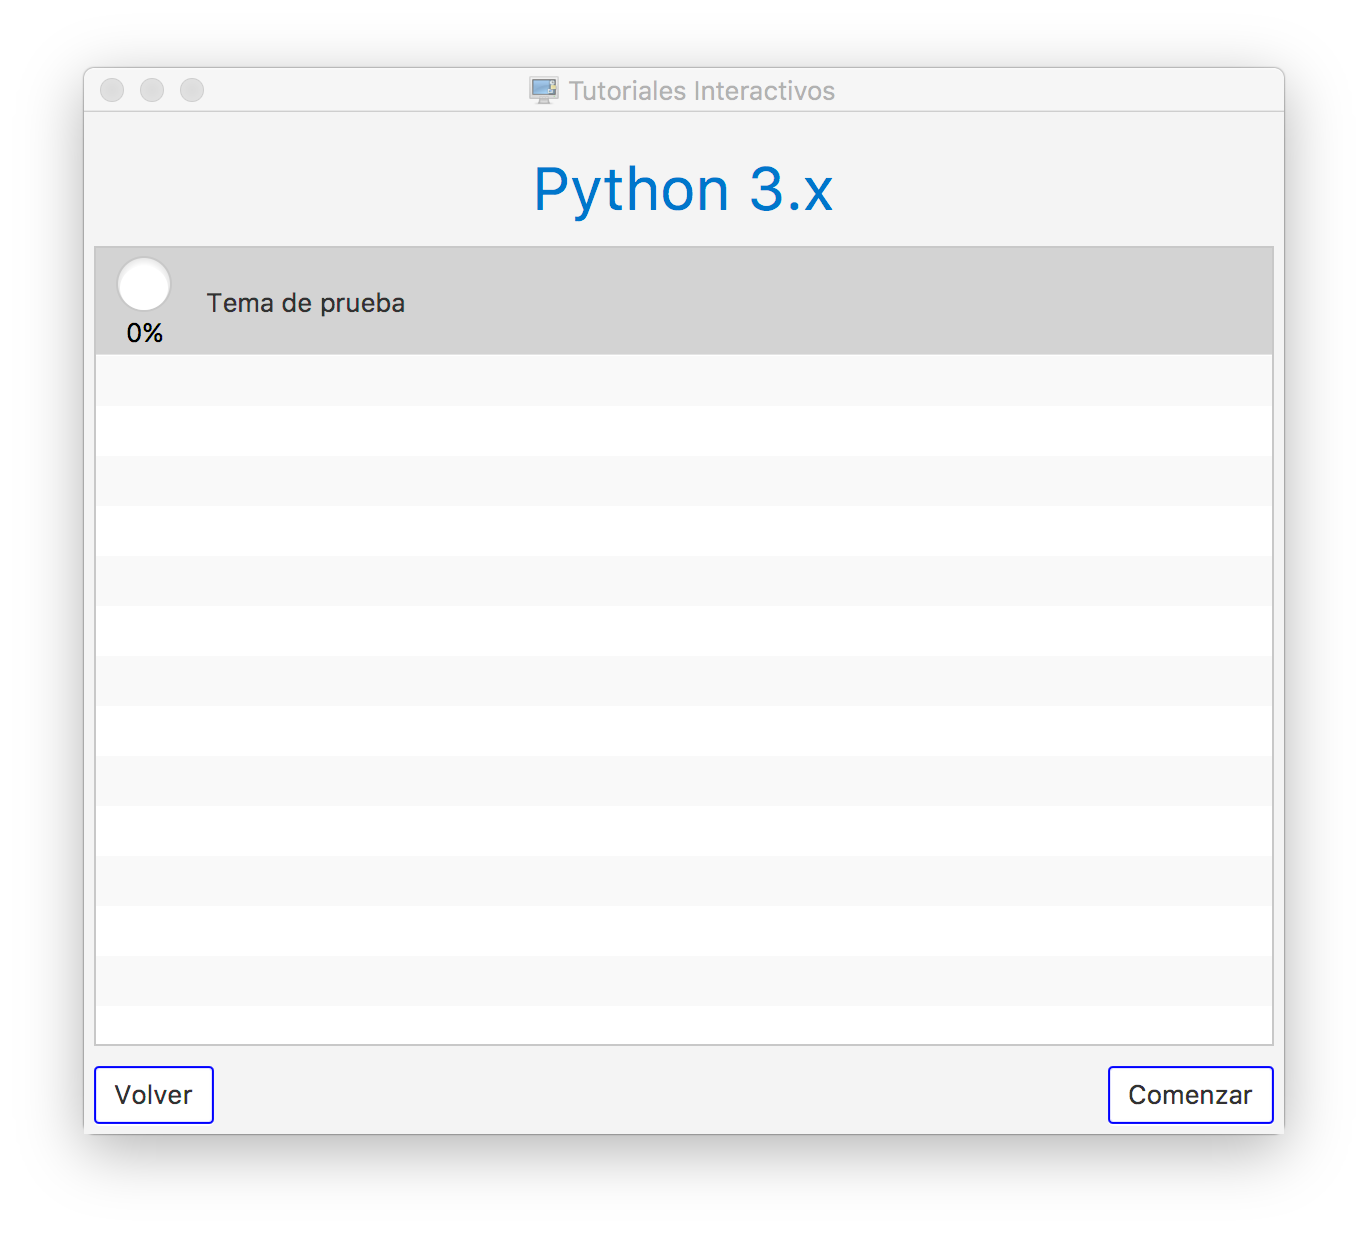
\includegraphics[scale=0.35]{ng_2.png}
\end{center}
\caption{Ventana de selección de temas\label{fig:ng_2}}
\end{figure}
%

%
\begin{figure}[tbp]
\begin{center}
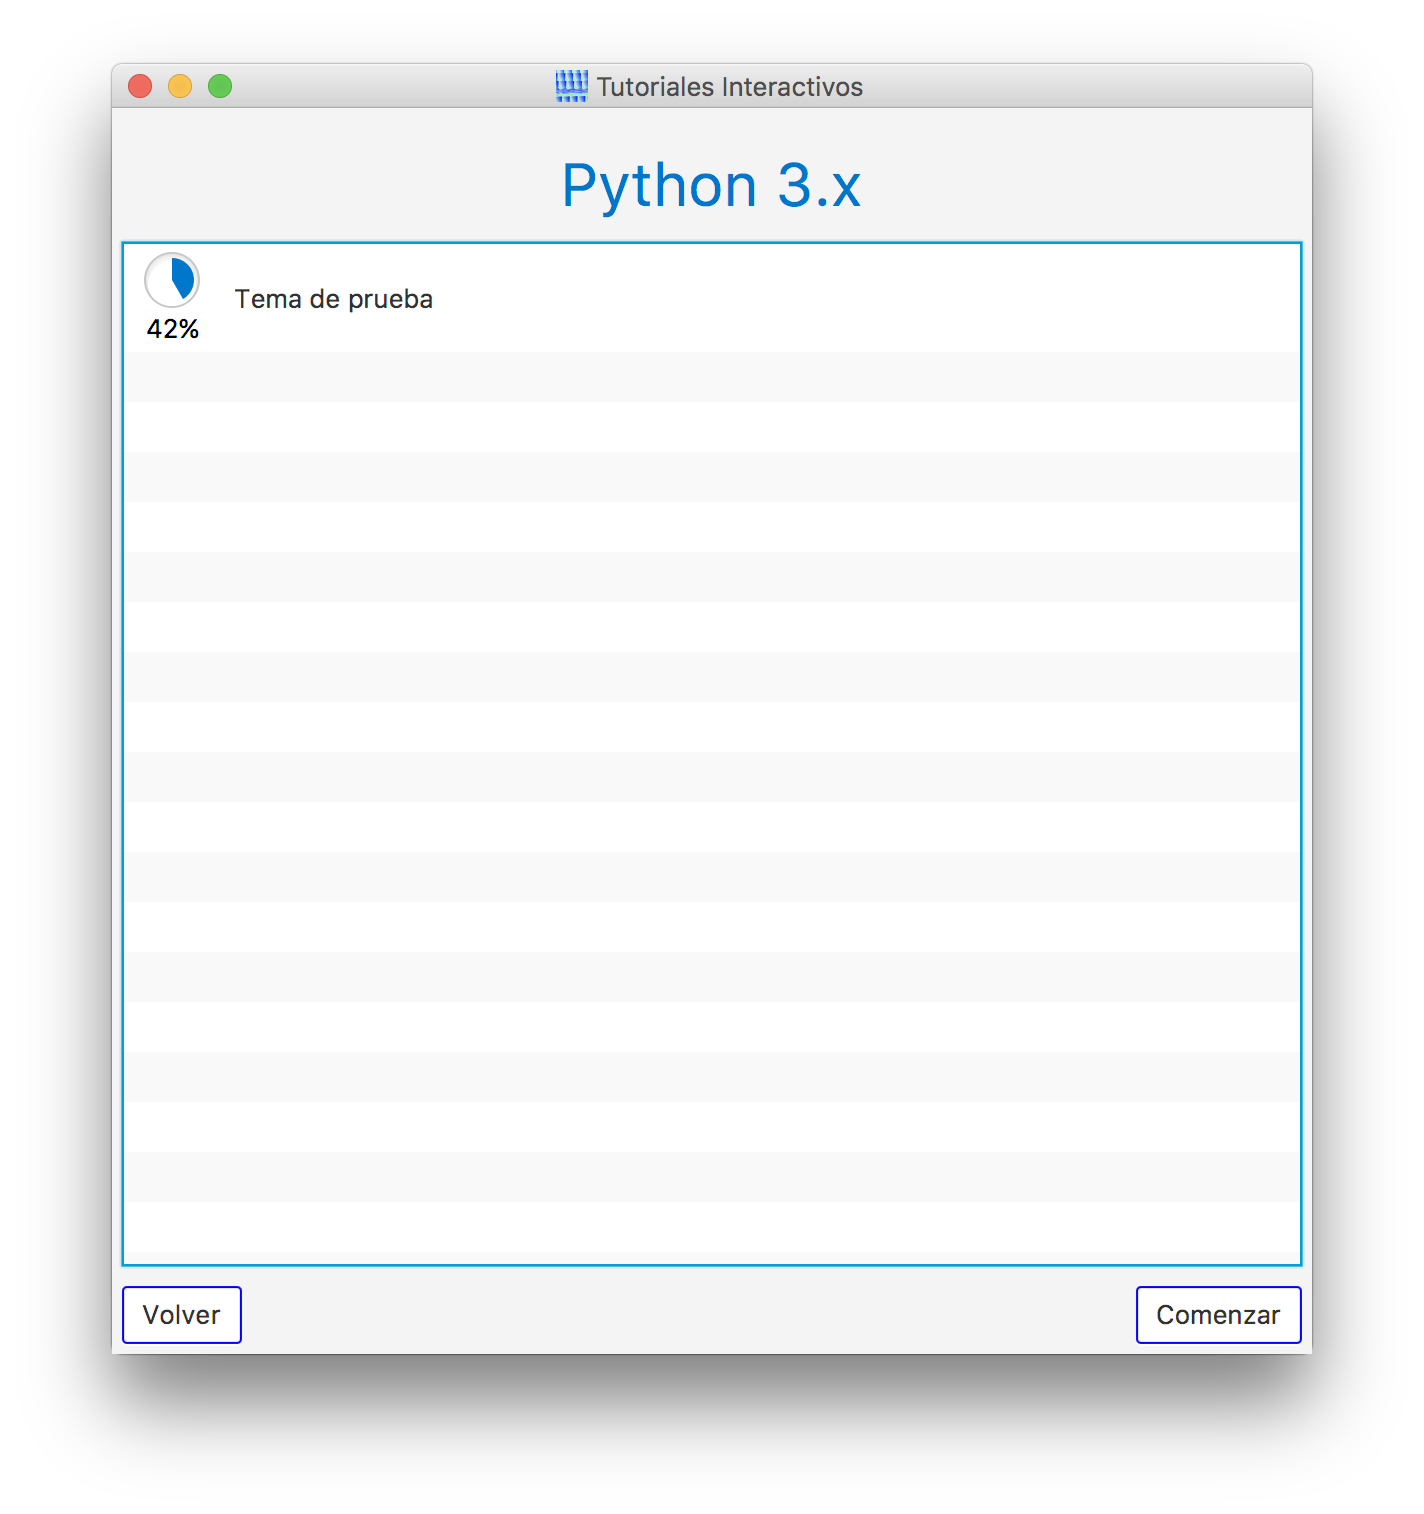
\includegraphics[scale=0.35]{ng_3.png}
\end{center}
\caption{Ventana de selección de temas tras completar parte de un tema\label{fig:ng_3}}
\end{figure}
%

\section{Lecciones}\todo{Tama}

Una vez seleccionado un tema, como se describe en la sección \ref{sec:ng}, entraremos en la selección de lecciones. Esta ventana tiene el aspecto que muestra la figura \ref{fig:l_1}. En este caso se dispone de tres lecciones, y para poder acceder a una de ellas la seleccionaremos y pulsaremos sobre el botón \emph{Comenzar lección}. También tendremos acceso a la ventana de selección de temas mediante el botón \emph{Menú anterior}. De manera similar a como ocurría para los temas, aquí también podremos observar el progreso en cada lección mediante el tanto por ciento mostrado a la parte izquierda de cada lección. Podemos ver un ejemplo de como se muestra este progreso en la figura \ref{fig:l_2}.

%
\begin{figure}[tbp]
\begin{center}
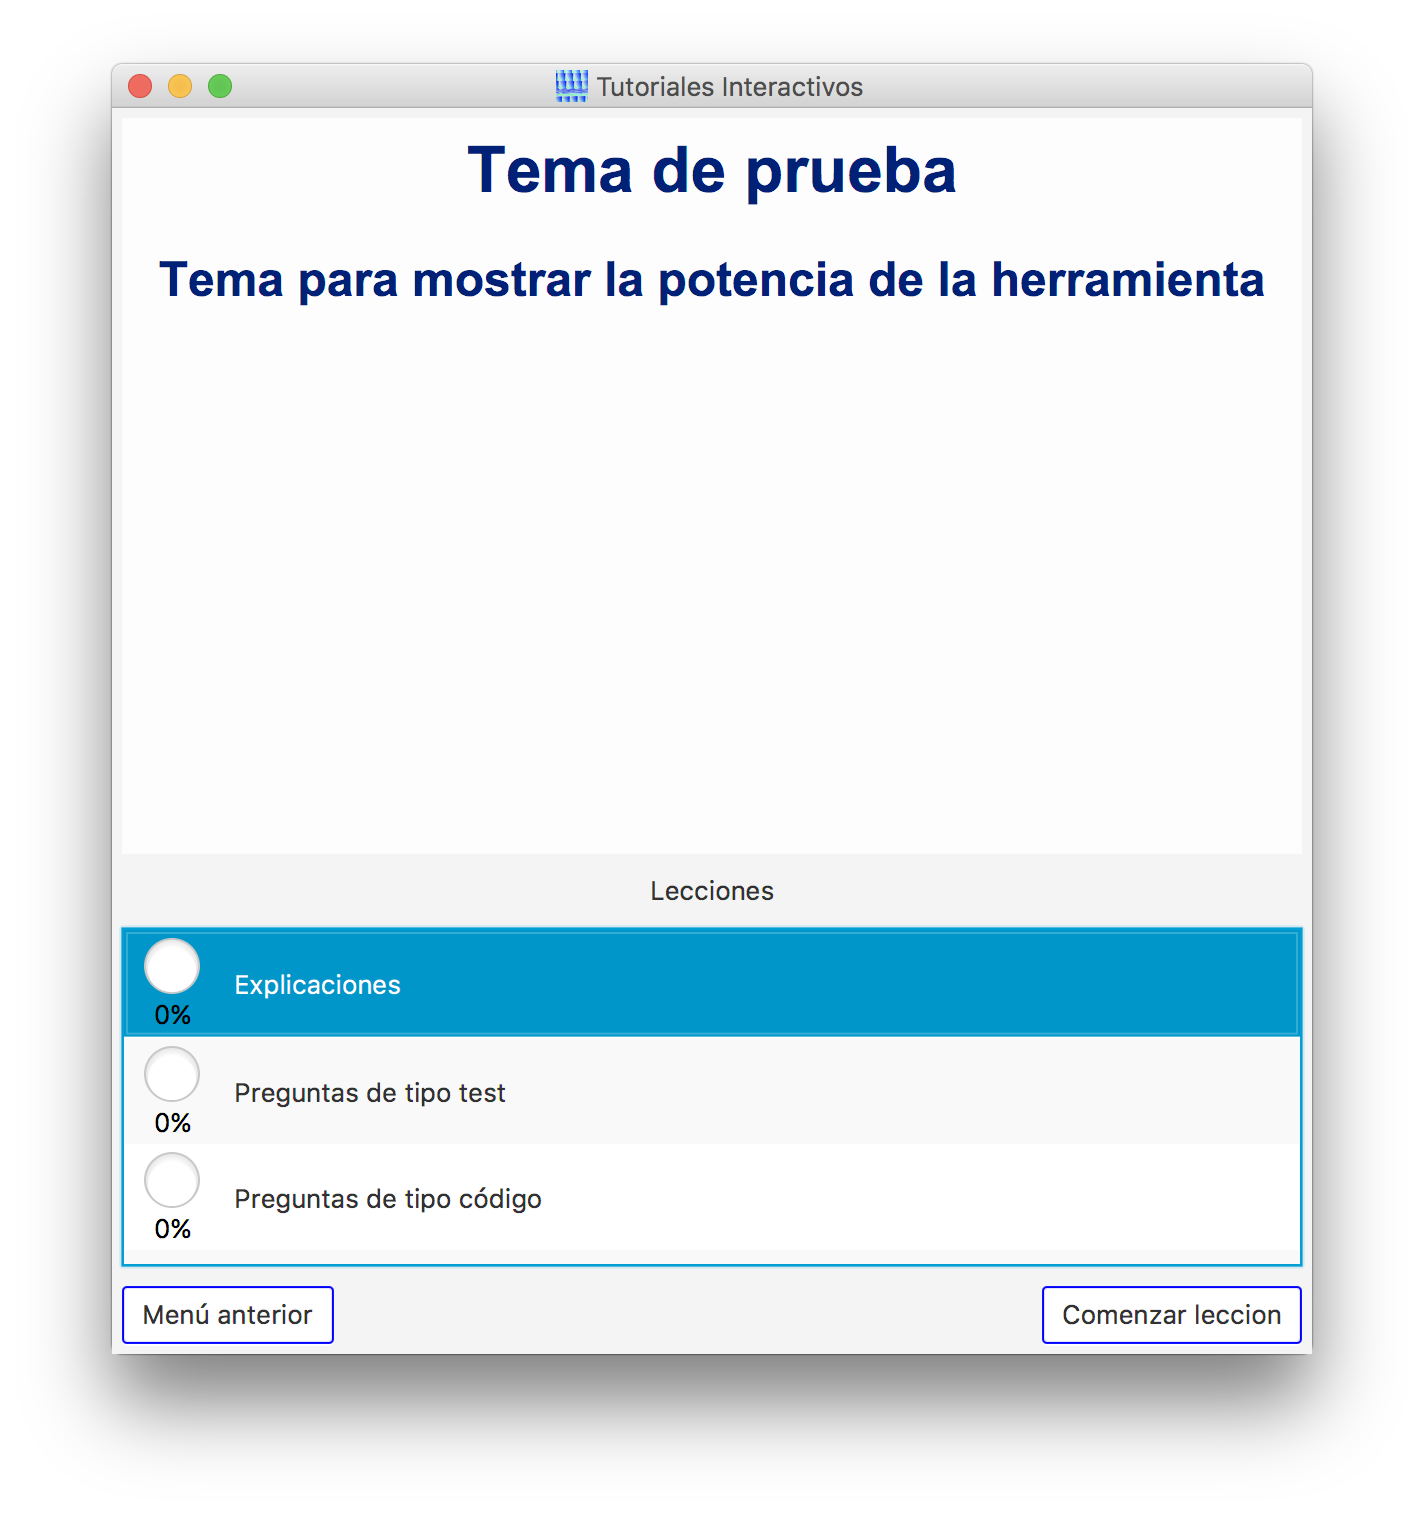
\includegraphics[scale=0.35]{l_1.png}
\end{center}
\caption{Ventana de selección de lecciones\label{fig:l_1}}
\end{figure}
%

%
\begin{figure}[tbp]
\begin{center}
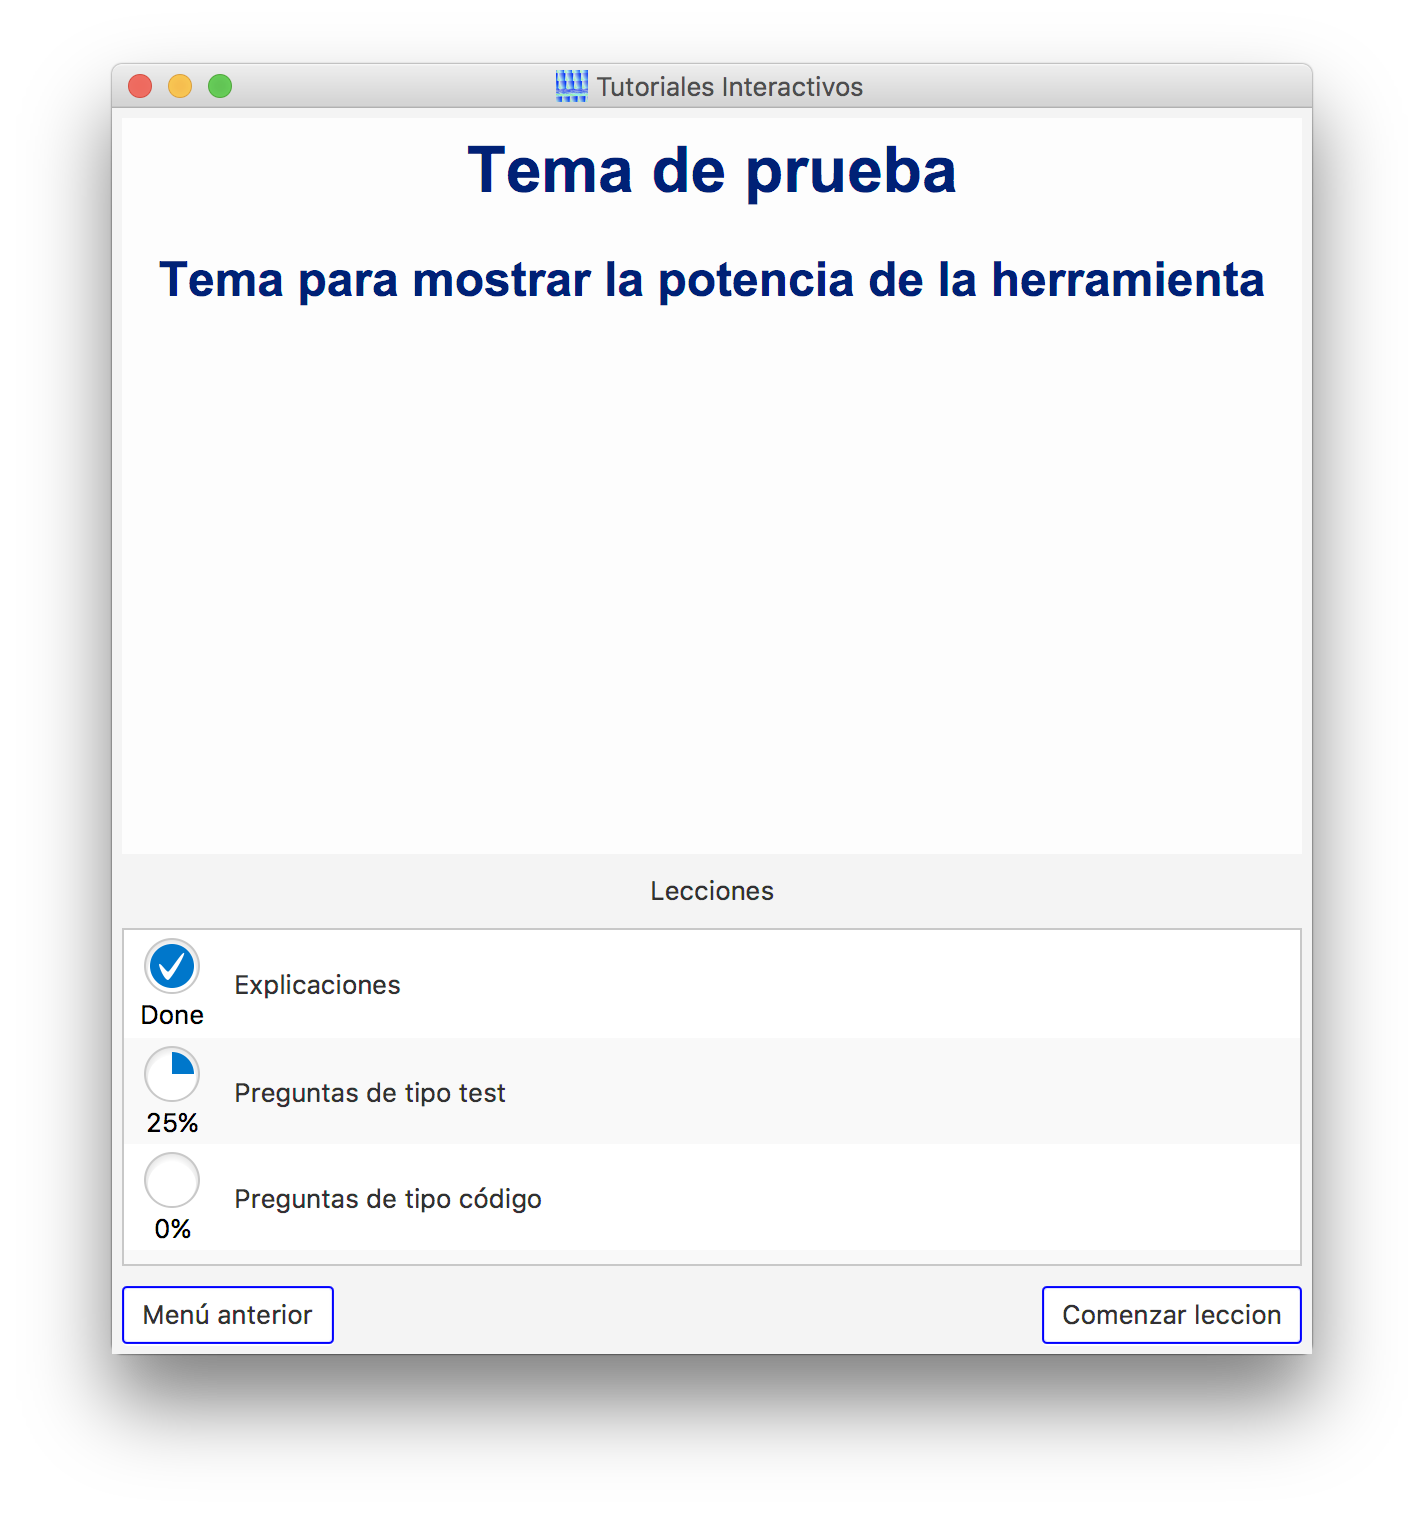
\includegraphics[scale=0.35]{l_2.png}
\end{center}
\caption{Ventana de selección de lecciones con algunos avances\label{fig:l_2}}
\end{figure}
%

Una vez dentro de una lección, veremos una ventana como la mostrada en la figura \ref{fig:l_3}. En esta ventana podemos observar varios elementos. Por una parte se nos mostrará en la parte superior toda la información sobre la lección cargada, i.e. el lenguaje, el tema y el nombre de la lección. El siguiente elemento es una descripción del problema, una pregunta o incluso una explicación. En caso de ser uno de los dos primeros, el usuario deberá resolver el ejercicio, y para ello tendrá un campo para incluir la respuesta. Este campo incluye un botón \emph{Resolver} para comprobar si la respuesta es correcta y, a veces, un botón \emph{Pistas}, para obtener una serie de pistas que ayuden al alumno a resolver el ejercicio. Finalmente se podrá navegar por las lecciones mediante los botones \emph{$<<$ Anterior}, siempre que no sea el primer ejercicio, o el botón \emph{Siguiente $>>$}, siempre que se haya resuelto el ejercicio que se muestre en el momento y éste no sea el último. Una manera alternativa de navegar por los ejercicios es mediante los números que identifican a cada ejercicio dentro de la lección. En este caso la restricción de haber resuelto los ejercicios también es necesaria para poder ir a ejercicios posteriores al actual. Finalmente, desde cualquier ejercicio podremos cambiar de tema o de lección mediante los botones \emph{Elegir tema} y \emph{Elegir lección} respectivamente.  

%
\begin{figure}[tbp]
\begin{center}
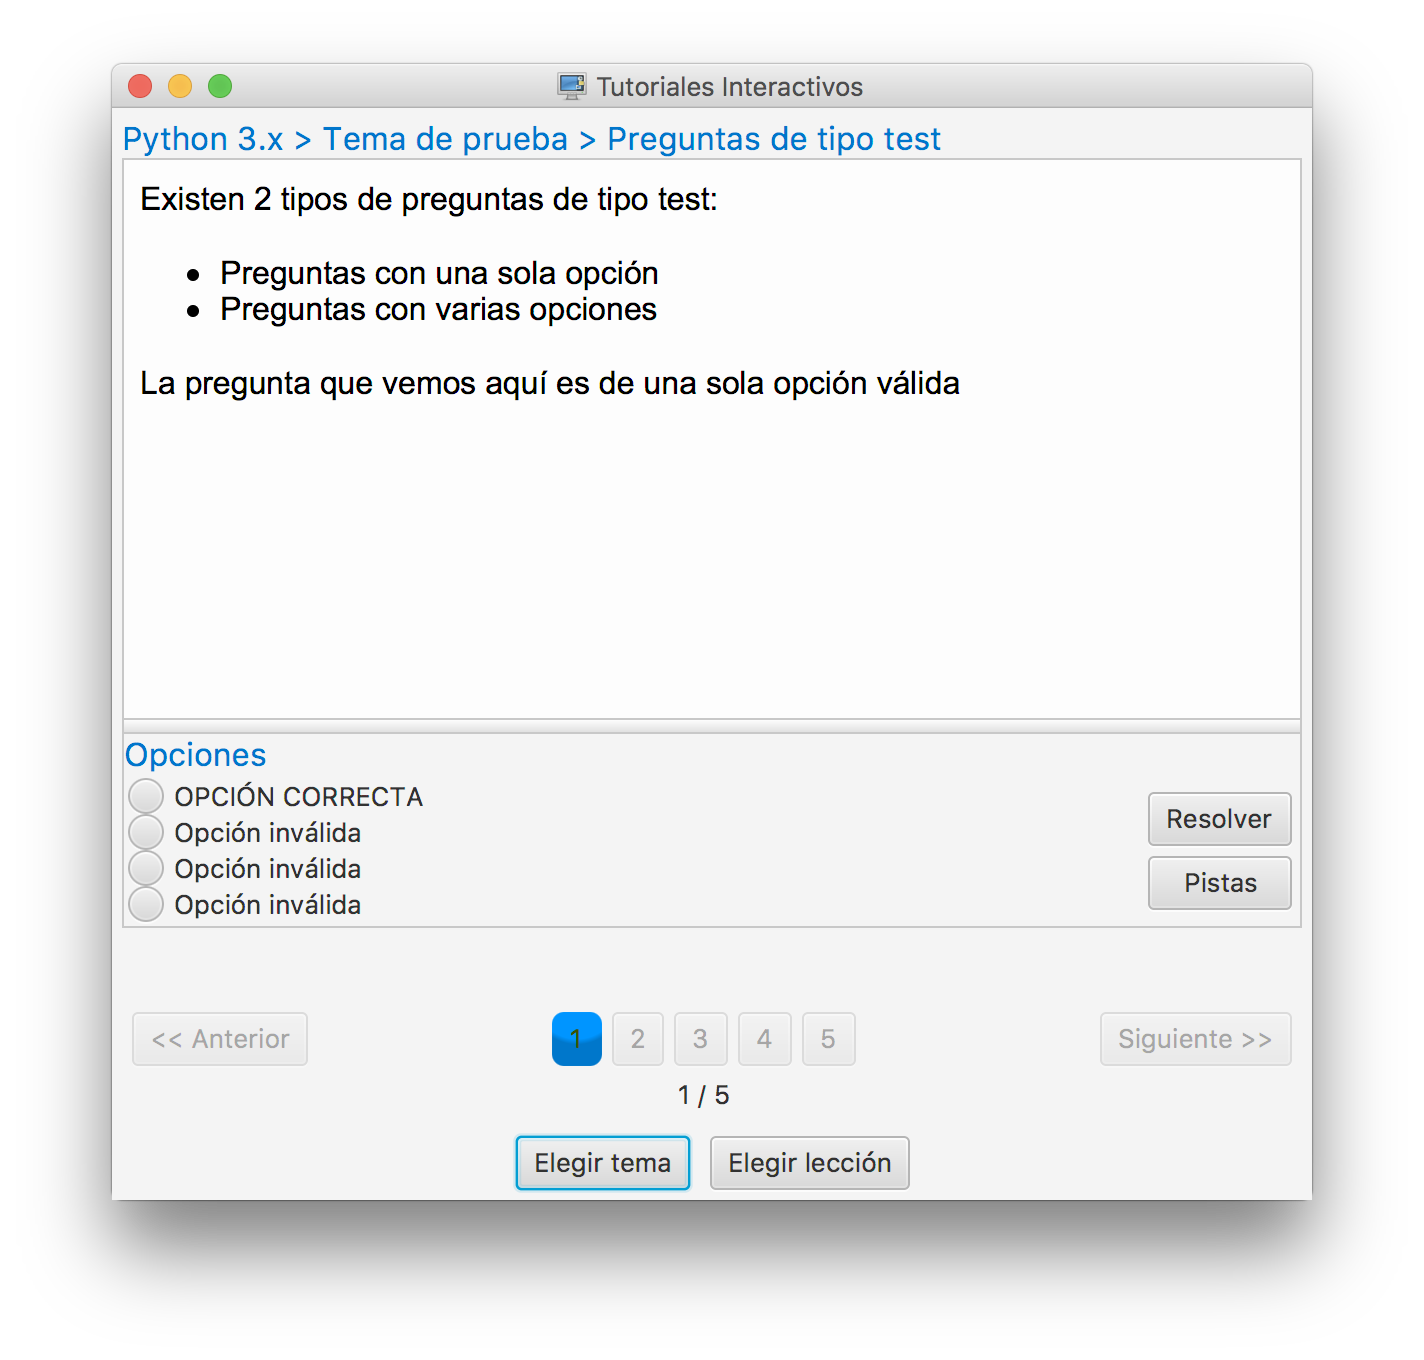
\includegraphics[scale=0.35]{l_3.png}
\end{center}
\caption{Ventana mostrando un ejercicio de una lección\label{fig:l_3}}
\end{figure}
%


La introducción de las respuestas depende del tipo de pregunta. Por ejemplo, en el caso del ejercicio mostrado en la figura \ref{fig:l_3}, solo hay una opción posible. Tras seleccionar la que creamos que sea la opción correcta, pulsaremos sobre el botón \emph{Resolver}, para comprobar si es correcta. En caso de ser incorrecta, se nos mostrará \emph{RESPUESTA INCORRECTA} sobre un fondo rojo, y deberemos, por tanto, cambiar la respuesta y volver a pulsar sobre el botón \emph{Resolver}. Cuando la respuesta sea correcta se mostrará \emph{CORRECTO} sobre un fondo verde,  como podemos ver en la figura \ref{fig:l_4}, y se habilitará el botón \emph{Siguiente $>>$}, siempre que no sea el último ejercicio de la lección. De manera similar, se habilitará el botón correspondiente al siguiente ejercicio, en este caso el número 2. 

%
\begin{figure}[tbp]
\begin{center}
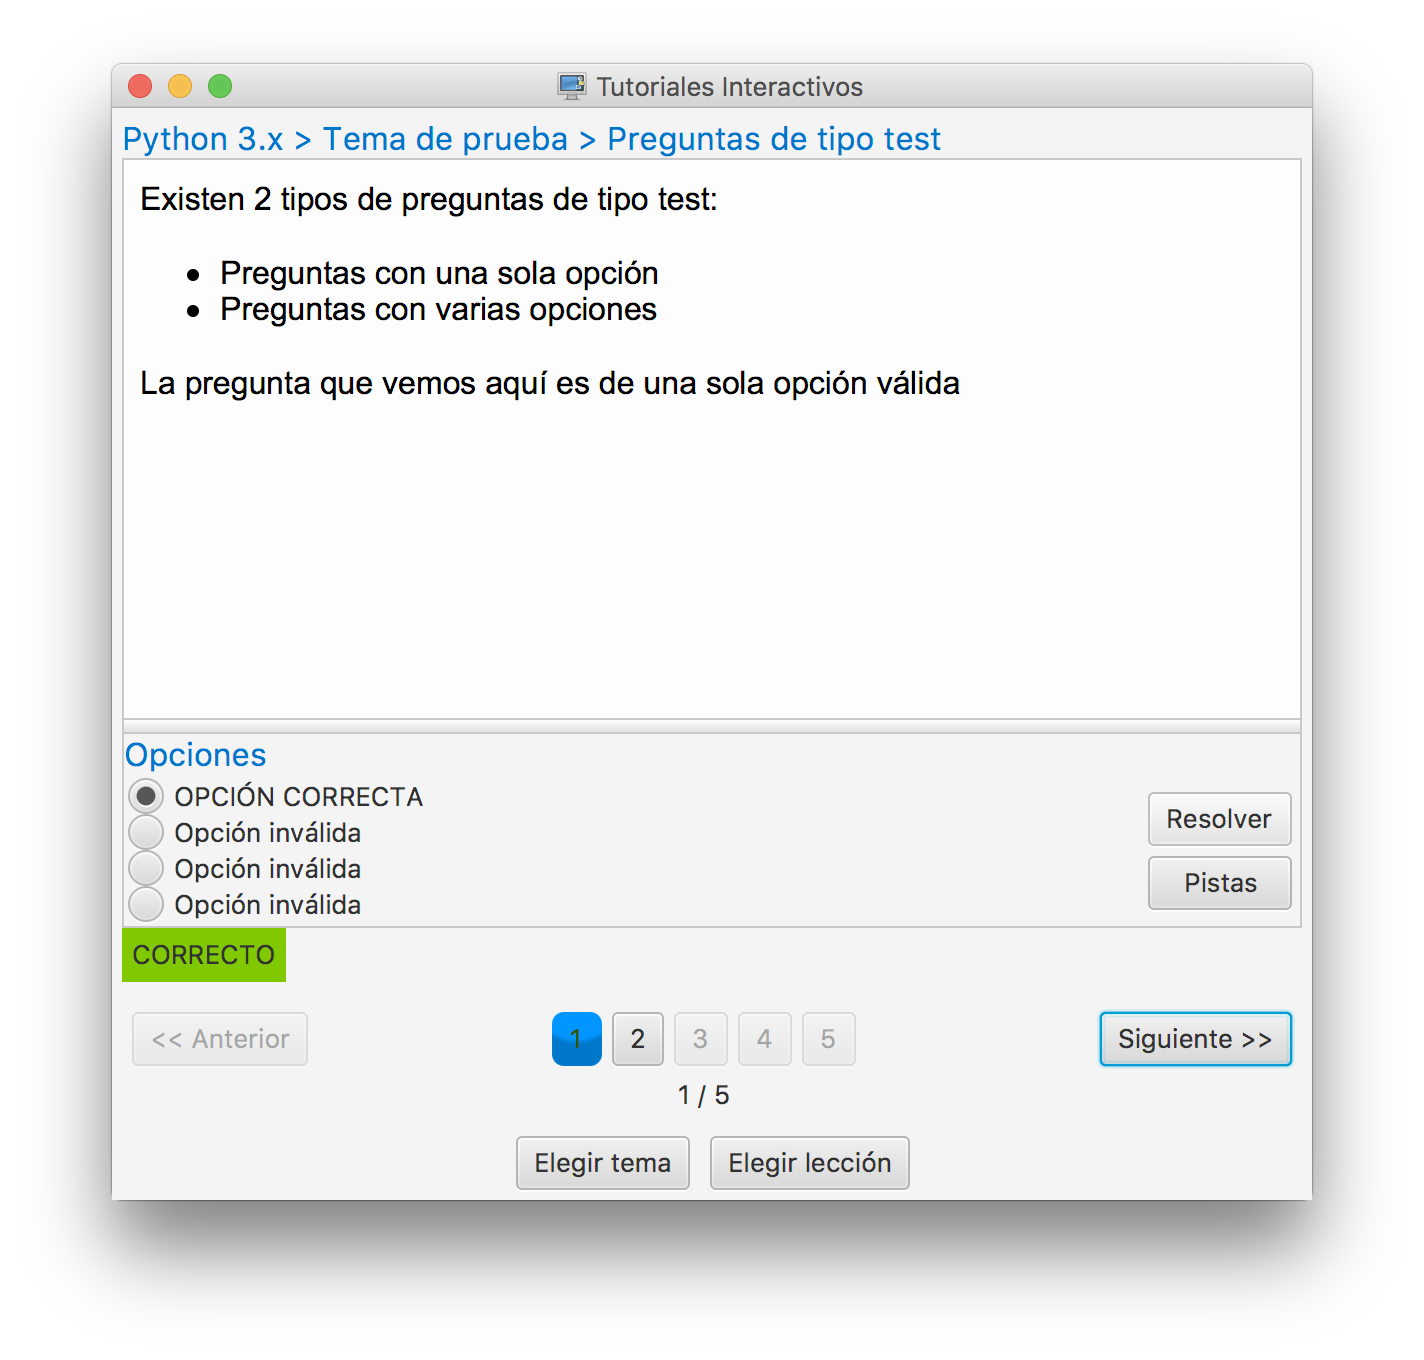
\includegraphics[scale=0.35]{l_4.png}
\end{center}
\caption{Ventana mostrando un ejercicio de una lección tras resolver el ejercicio\label{fig:l_4}}
\end{figure}
%

Otros tipos de respuestas que nos podemos encontrar son en las que existen varias opciones seleccionables, como se muestra en la figura \ref{fig:l_5}. En este caso se seleccionarán las opciones que se consideren correctas (puede que no sea ninguna) y se pulsará sobre el botón \emph{Resolver} para conocer el resultado. También existen ejercicios de desarrollo, donde el alumno deberá de introducir su respuesta mediante un campo de texto. Un ejemplo de estos ejercicios el que se muestra en la figura \ref{fig:l_6}. En estos tipos de ejercicios, además se incluye el botón \emph{Borrar}, para borrar los campos de texto de la respuesta. Tras introducir la respuesta el alumno deberá pulsar el botón \emph{Resolver} para conocer si es correcta o no. A veces estos ejercicios de desarrollo vienen con varios huecos a completar por el alumno, como, por ejemplo, el mostrado en la figura \ref{fig:l_7}. El modo de proceder es exactamente igual que el anterior. En estos casos, además se incluye el botón \emph{Ver código}, que permite ver el aspecto del código con la respuesta introducida hasta el momento. Finalmente, al llegar al final de la lección se nos mostrará una ventana como la de la figura \ref{fig:l_8} desde la cual podremos revisar los ejercicios de la lección, acceder a una nueva mediante el botón \emph{Elegir lección} o cambiar de tema con el botón \emph{Elegir tema}. 

%
\begin{figure}[tbp]
\begin{center}
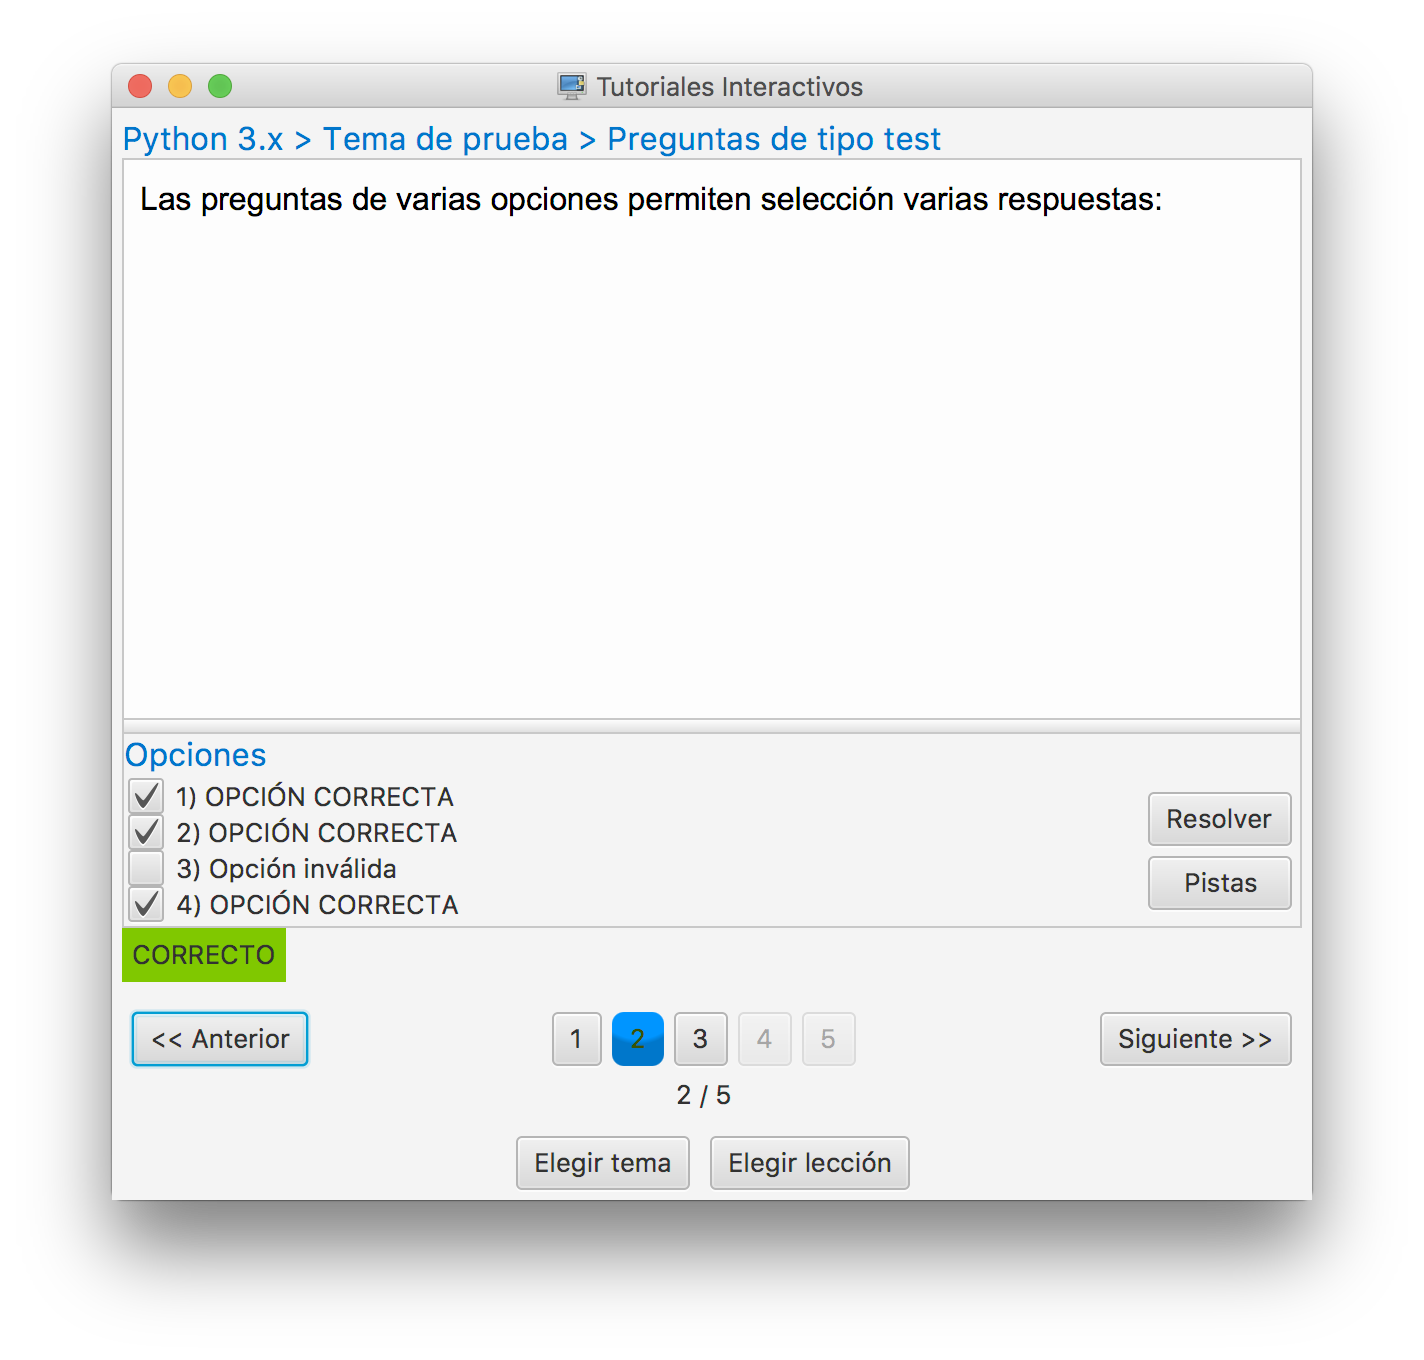
\includegraphics[scale=0.35]{l_5.png}
\end{center}
\caption{Ventana mostrando un ejercicio con multiples opciones seleccionables\label{fig:l_5}}
\end{figure}
%

%
\begin{figure}[tbp]
\begin{center}
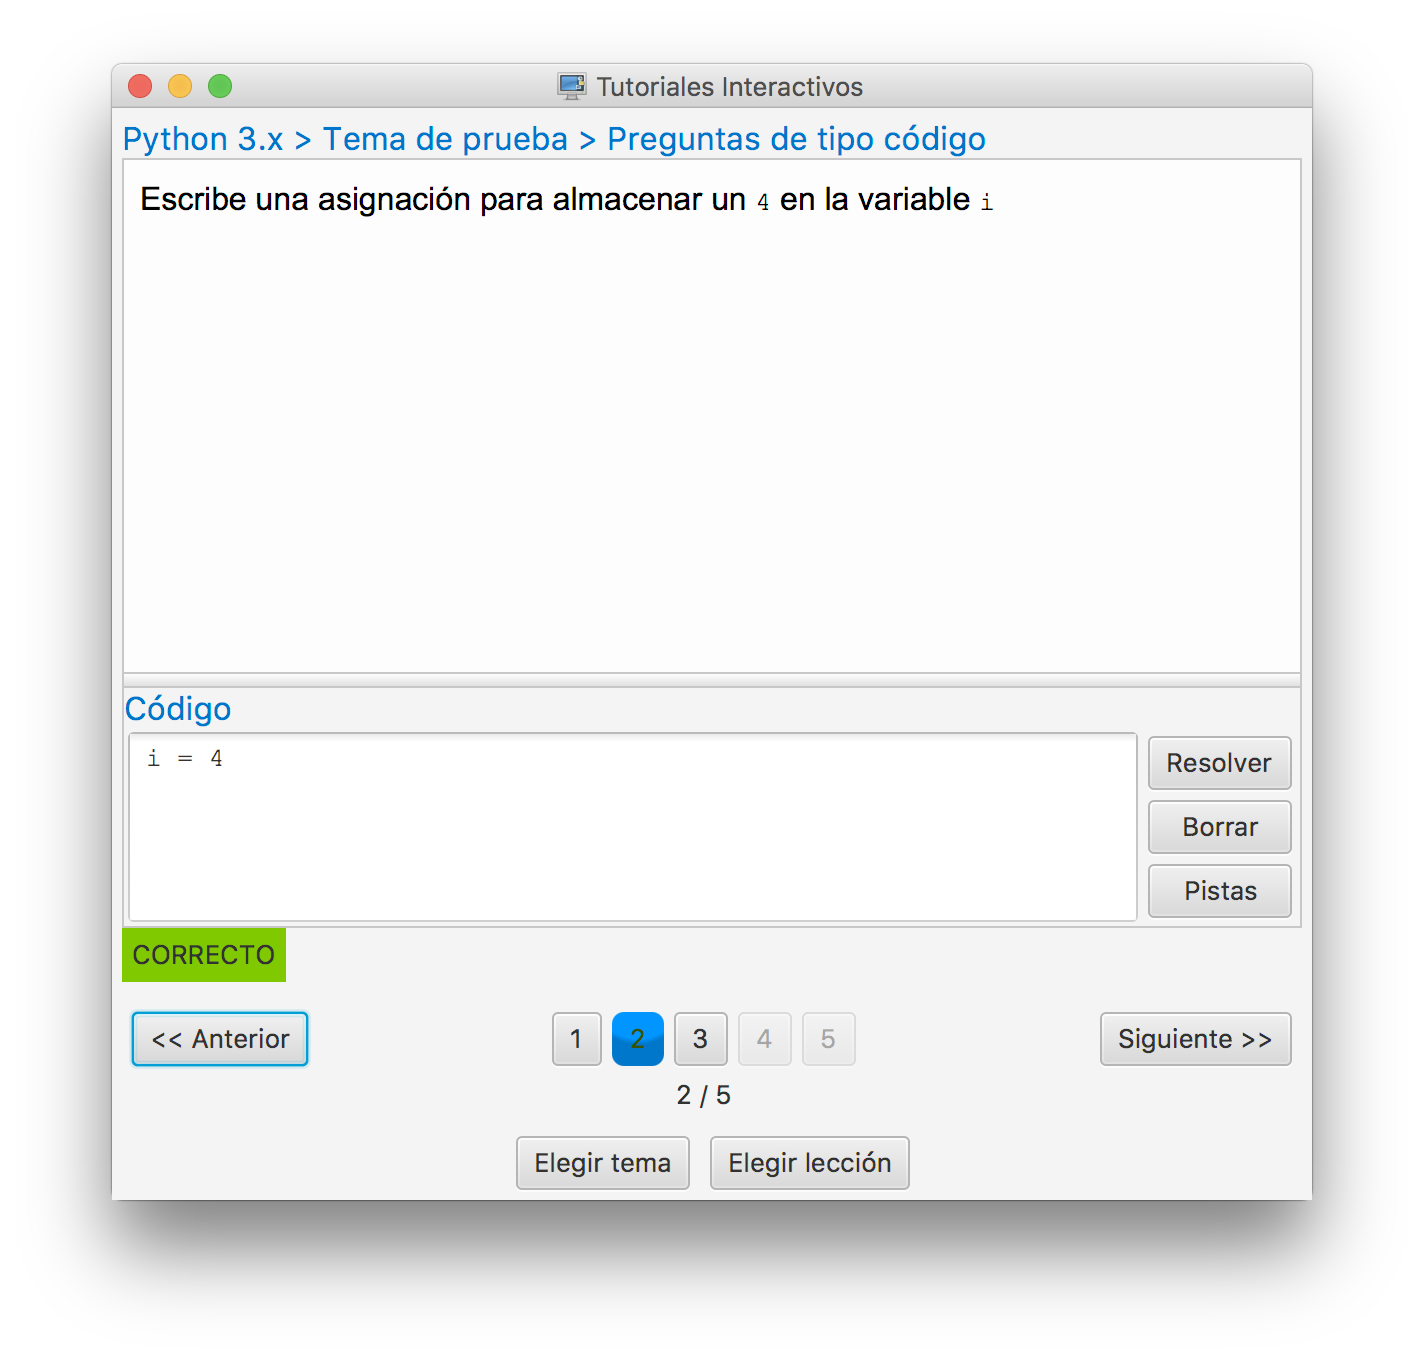
\includegraphics[scale=0.35]{l_6.png}
\end{center}
\caption{Ventana mostrando un ejercicio con un ejercicio de desarrollo\label{fig:l_6}}
\end{figure}
%

%
\begin{figure}[tbp]
\begin{center}
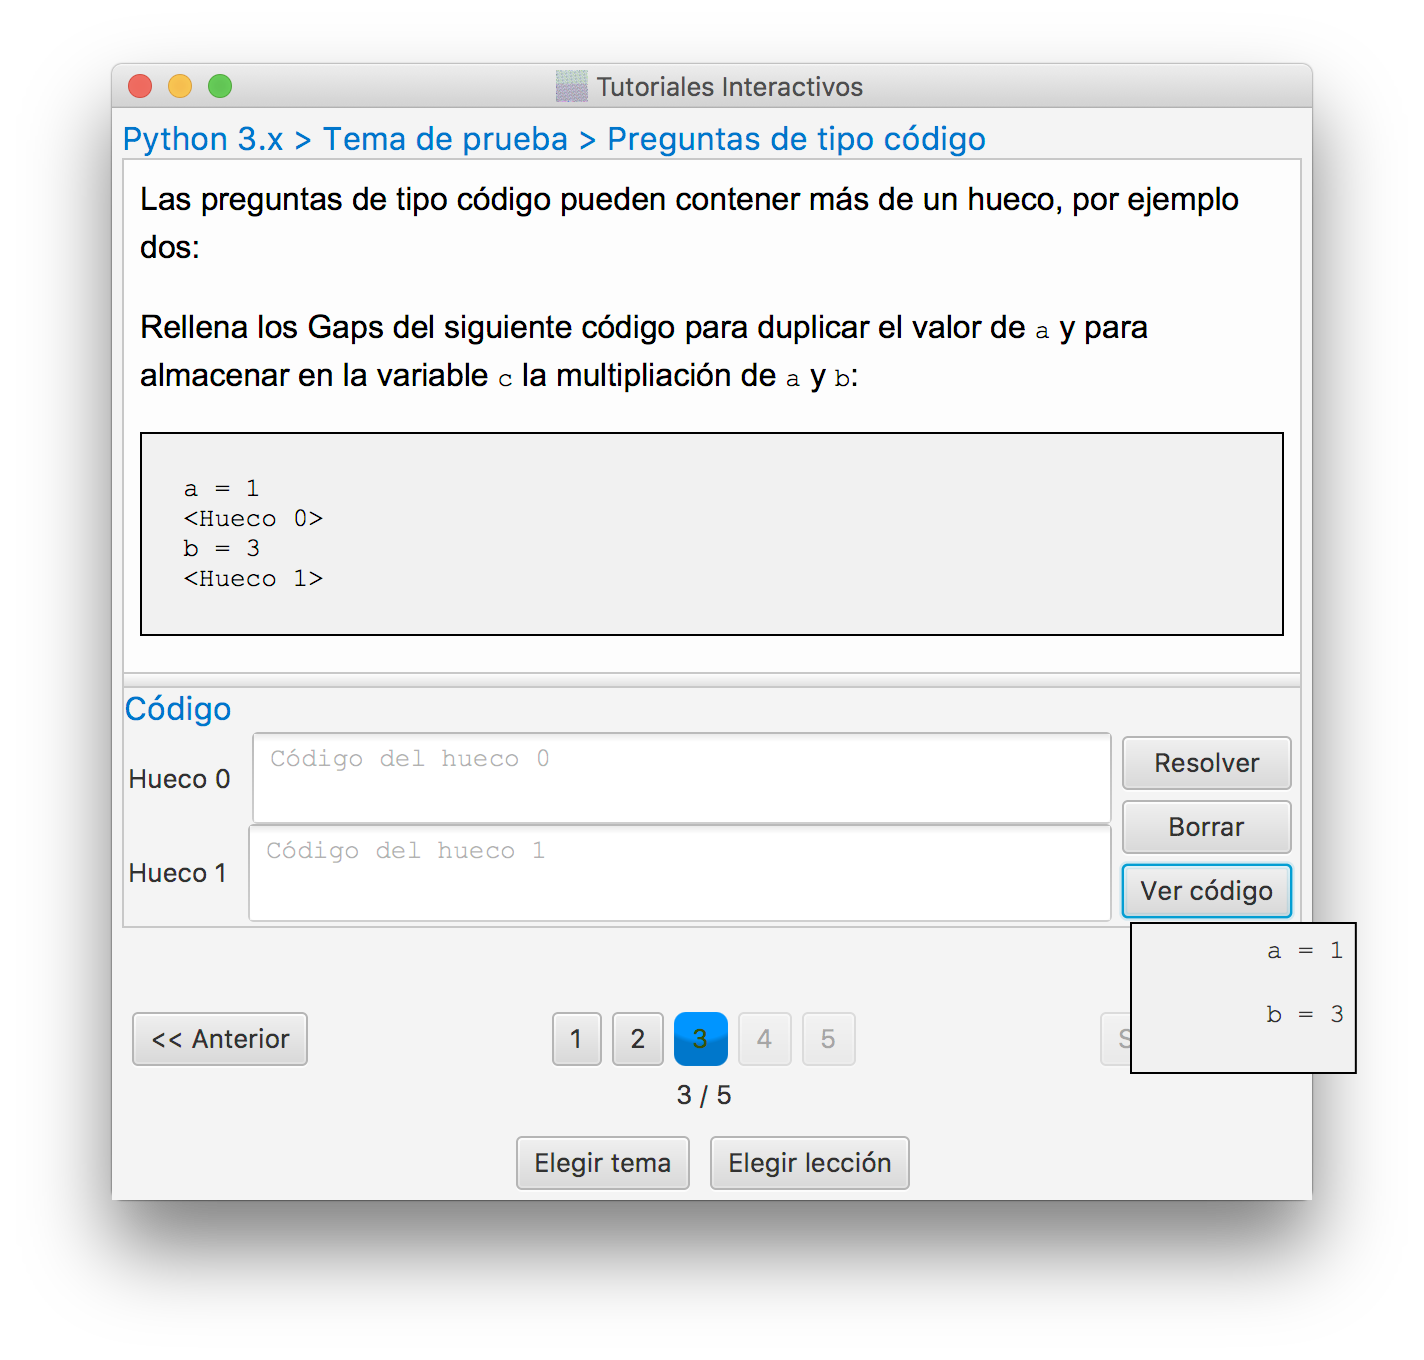
\includegraphics[scale=0.35]{l_7.png}
\end{center}
\caption{Ventana mostrando un ejercicio con un ejercicio de desarrollo con varios huecos a rellenar\label{fig:l_7}}
\end{figure}
%

%
\begin{figure}[tbp]
\begin{center}
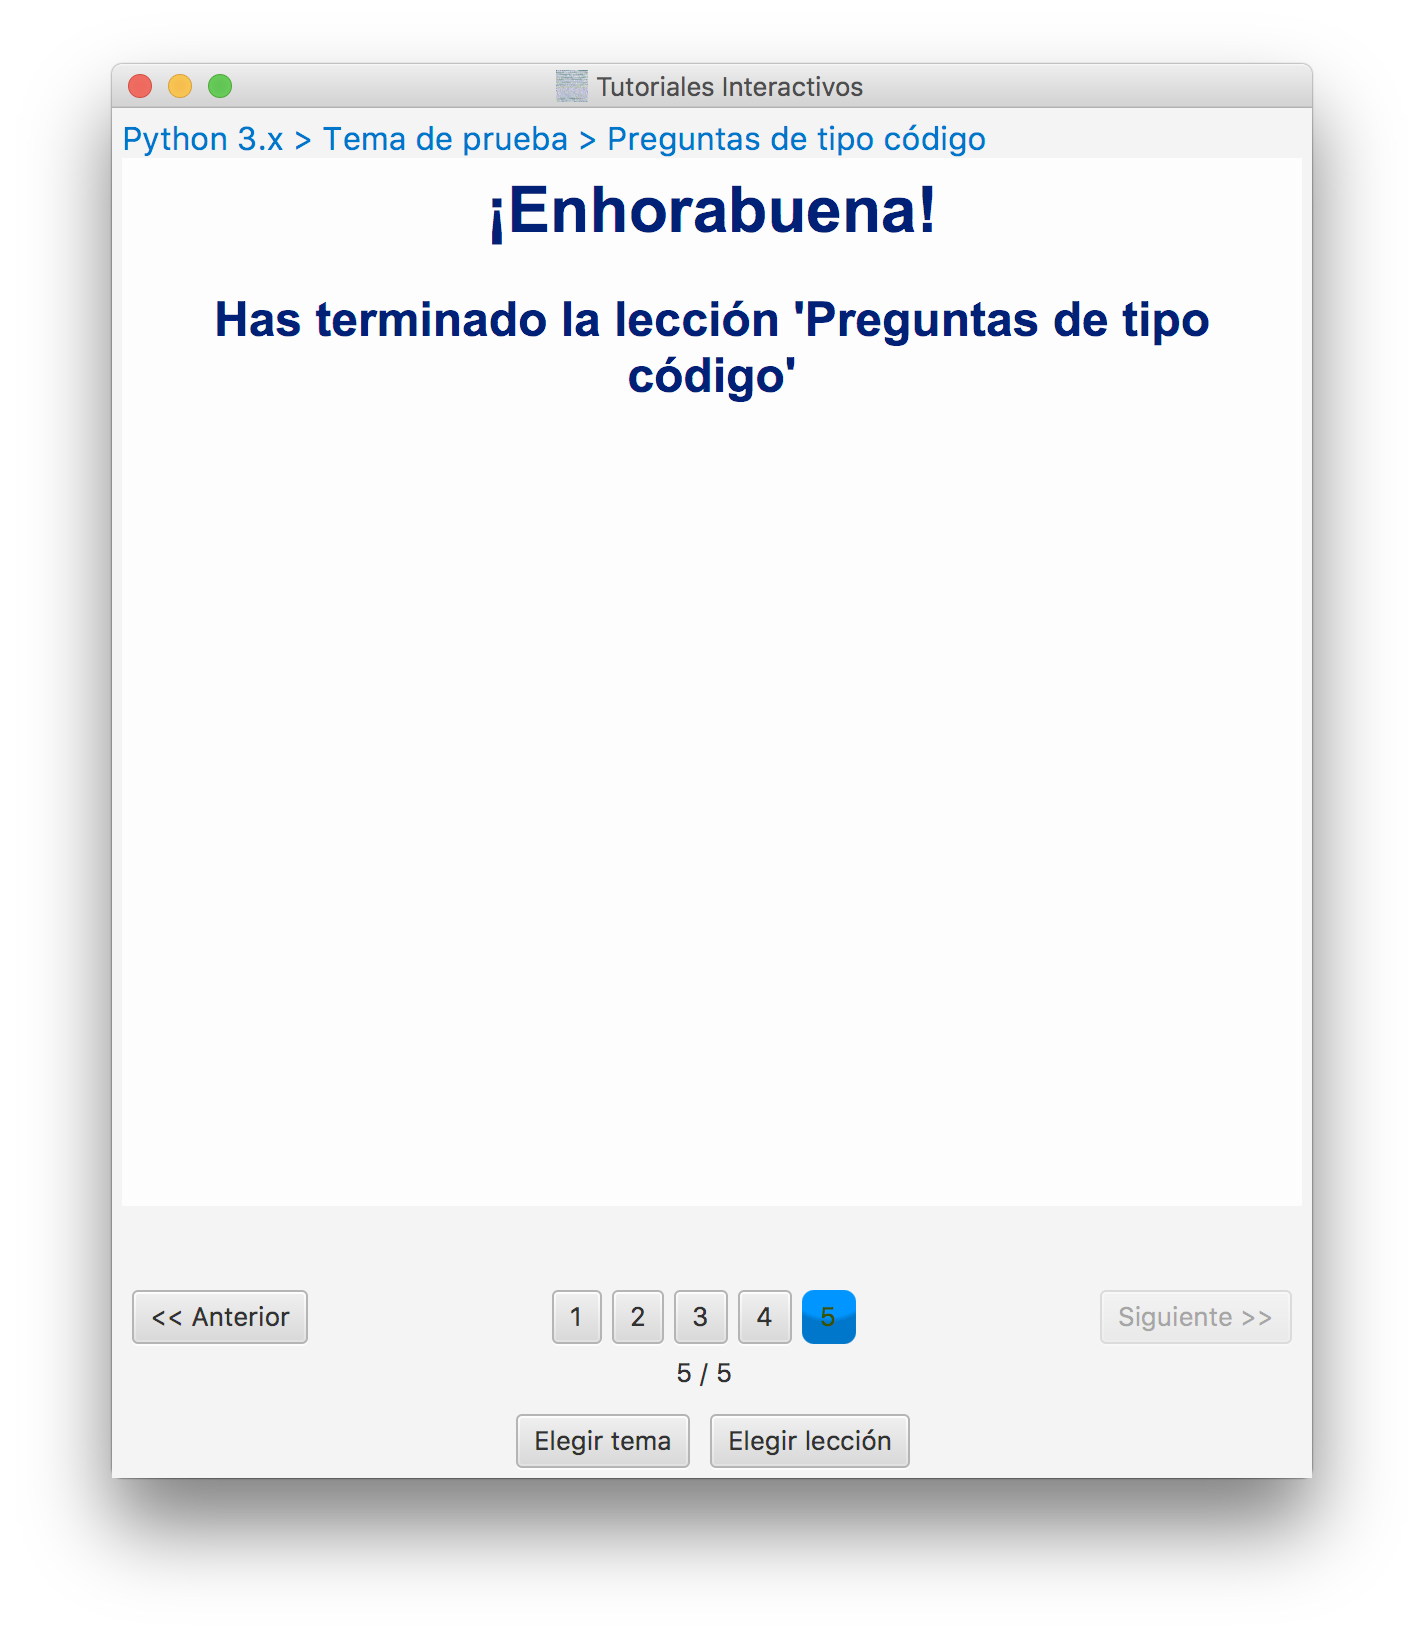
\includegraphics[scale=0.35]{l_8.png}
\end{center}
\caption{Última ventana correspondiente a una lección\label{fig:l_8}}
\end{figure}
%

\section{Solución de problemas}\todo{Enrique}

\subsection{No puedo iniciar la herramienta}\label{sec:problemas_arrancar}
Si al hacer doble clic sobre el fichero \texttt{.jar} no se arranca la aplicación, comprueba que dicho fichero es \textbf{ejecutable}. Para ello abre el menú contextual con el botón derecho y explora las distintas opciones disponibles para cambiar los permisos del fichero.

Si aún así los problemas persisten, prueba alguna de las siguientes opciones:
\begin{itemize}
	\item \textbf{En sistemas Windows}: 
	\begin{itemize}
	\item Haz doble clic en el fichero \texttt{TutorialesInteractivos.bat} que está en el directorio \textbf{principal} de la herramienta. 
	\item Abre un teminal (\emph{Command Prompt}), dirígete al directorio principal de la herramienta y ejecuta alguno de estos comandos:
	\\
	{\small \texttt{>\ TutorialesInteractivos.bat}}\\
	{\small \texttt{>\ java -jar target/TutorialesInteractivos-jar-with-dependencies.jar}}\\
	\end{itemize}
	\item \textbf{En sistemas Linux y Mac}:
	\begin{itemize}
		\item Haz doble clic en el fichero \texttt{TutorialesInteractivos.sh} que está en el directorio \textbf{principal} de la herramienta. 
		\item Abre un teminal, dirígete al directorio principal de la herramienta y ejecuta alguno de estos comandos:
		\\
		{\small \texttt{\$ TutorialesInteractivos.sh}}\\
		{\small \texttt{\$ java -jar target/TutorialesInteractivos-jar-with-dependencies.jar}}\\
	\end{itemize}
\end{itemize}	
	
%	 doble clic en target/blablabla.jar, lanzar .sh desde Command Prompt
%	\item Mac: doble clic en target/blablabla.jar, lanzar .sh desde Command Prompt


\subsection{La herramienta se inicia con errores}
Si la herramienta se inicia con errores o tiene un comportamiento anómalo, lo mejor es limpiar todas las configuraciones y empezar desde cero. Para ello existe una opción \texttt{--reset} que se puede utilizar al invocar a la aplicación. Para ello abre un terminal y, dentro del directorio principal de la aplicación, ejecuta el siguiente comando:\\[0.2cm]
{\small \texttt{java -jar target/TutorialesInteractivos-jar-with-dependencies.jar --reset}}\\[0.2cm]
La herramienta eliminará todos los valores almacenados en ejecuciones previas (directorio de temas, rutas de compiladores/intérpretes y progreso dentro de cada lección) y se iniciará como si fuese la primera vez. 

\end{document}          
